\chapter{Background in optimal control problems\\}
\label{cha:3}

This chapter gives some background information of the theory behind optimal control (OCP). After a global introduction and the discussion about the time discretization and shooting option, the chapter is being specified into model predictive control (MPC).\\

\subsection{Optimal control problem (OCP)}
An optimal control problem determines the desired inputs and corresponding state trajectories to change the system from an initial state to a desired final state in an optimal way while satisfying some input and state constraints \cite{Mercy2018}.

\begin{equation}
\label{eq:OCP}
\begin{aligned}
\min_{\bm{q}(.),\bm{u}(.)} \quad & \int_{0}^{T}l(\bm{q}(t),\bm{u}(t))dt + E(\bm{q}(T)) \\
\textrm{s.t.} \quad & \bm{\dot{q}}(t) = \bm{f}(\bm{q}(t), \bm{u}(t))\\
& \bm{q}(0)= \bm{q}_{0},\hspace{2 mm}\bm{q}(T)= \bm{q}_{T}    \\
& h(\bm{q}(t),\bm{u}(t)) \geq 0	\\
& \bm{q}(t)\in Q,\hspace{3 mm} \bm{u}(t)\in U, \hspace{3 mm} t\in [0, T]
\end{aligned}
\end{equation}

$\bm{q}$ is called contains all the states of the system and $\bm{u}$ containing the controls. In the context of vehicle control states are often kinematic variables like positions and velocities of the centre of gravity of the vehicle. $\bm{u}$ is containing the controls which are typically steerwheelangle and the amount of throttle which can be directly linked the amount of propulsion force. The objective function $l$ of the optimization problem is integrated over the desired control horizon $T$. The objective function indicates what should be minimized and is a function of the different states and controls. The terminal cost is represented by $E(\bm{q}(T))$ and can be needed to assure certain conditions of the system at the end of the control horizon. $\bm{\dot{q}}(t)$ describes the dynamics of the system by an explicit ordinary differential equation. Furthermore there are also constraints possible on states and inputs, represented by $h$, $Q$ and $U$ respectively. The results that come out of an OCP indicate which states will be visited by the system and which controls have to be applied in order to do this with respect to the constraints on an optimal manner. \cite{Patrinos2019}\\ 

There is a difference between soft and hard constraints. Soft constraints are placed in the objective function $l$. If the constraint is better fulfilled a more optimal solution will be obtained. A hard constraint, represented by $h$ in equation \ref{eq:OCP}, is explicitly put in the constraints and defines the feasible solution set of the optimization \cite{Yankov}.\\

\subsection{Time discretization}

The optimal control problem (equation \ref{eq:OCP}) is continuous in time which means that it has infinite dimensions. To be able to run the optimization problem on digital systems there is need for discretization. There are several ways to do this which are summarized in Figure \ref{fig:discretization_m}.
\begin{figure}[htp]
	\centering
	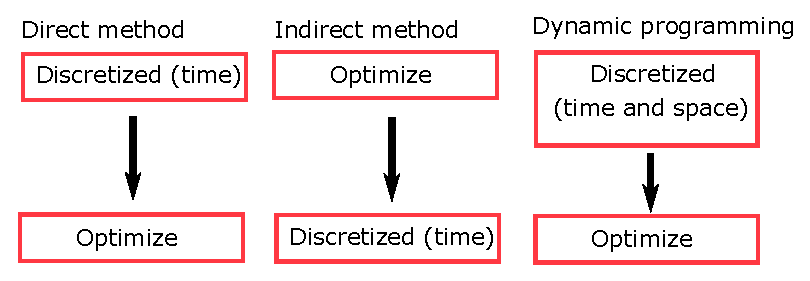
\includegraphics[width=0.8\textwidth]{discretized.eps}
	\caption{Overview of different discretization methods.}
	\label{fig:discretization_m}
\end{figure}

Since direct methods are best suited to solve practically relevant OCPs \cite{Mercy2018}, this thesis is following the direct method. To implement the discretization of time when using the Direct method, a time shooting approach can be used.

\subsubsection*{Time shooting}

A shooting approach makes use of a time grid. This means that time will be sampled and on every time instant the optimal control problem is assessed. Constraints will only be not violated on these time instants but no limits are set between different time samples. To bound the system to the constraints a high enough sampling rate is desired. \cite{Mercy2018}
Two different shooting approaches exist:\\
\begin{enumerate}
	\item Multiple shooting (MS)\\
	During multiple shooting $ns\in \mathbb{N}$ new states and $nc \in \mathbb{N}$ new controls are defined on every new time sample and are taken as optimization variables. Because input changes are only allowed on the time samples this will often lead to a piece wise control input signal. This is indicated by the blue bars in Figure \ref{fig:TS} (left). The red dots in Figure \ref{fig:TS} (left) indicate the condition of the states on the discrete time samples. In order to make the connection $\bm{q}(k+1) = \bm{f}(\bm{q}(k), \bm{u}(k))$ from the previous state to the next, time integration is used. The constraints introduced in this way are called in literature 'path closing constraints' \cite{Gillis2019}. \\
	
	\item Single shooting (SS)\\  
	In the single shooting or sequential approach only the initial state and control points are optimization variables. This is achieved by replacing the state variable by the integration result from the previous state \cite{Gillis2019}. This approach is show in equation \ref{eq:2}. Figure \ref{fig:TS} (right) gives a visualization with the green dots indicating the result of one integration step from the previous state.
	
	\begin{equation}\label{eq:2}
	\begin{aligned}
	\bm{q}(1) &= \bm{f}(\bm{q}(0), \bm{u}(0))\\
	\bm{q}(2) &= \bm{f}(\bm{f}(\bm{q}(0), \bm{u}(0)), \bm{u}(1))\\
	\bm{q}(3) &= \bm{f}(\bm{f}(\bm{f}(\bm{q}(0), \bm{u}(0)), \bm{u}(1)), \bm{u}(2))\\
	...
	\end{aligned}
	\end{equation}
\end{enumerate}
%\vspace{1 cm}

\begin{figure}[htp]
	\centering
	\begin{minipage}{0.49\textwidth}
		\centering
		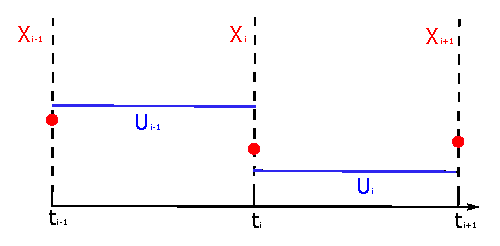
\includegraphics[width=1\textwidth]{MS_int.eps}
	\end{minipage}
	\hfill
	\begin{minipage}{.49\textwidth}
		\centering
		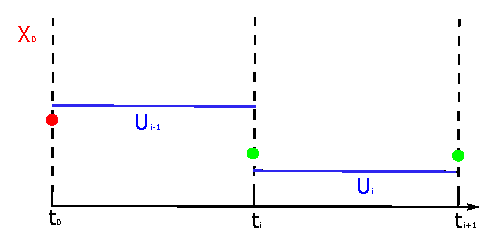
\includegraphics[width=1\textwidth]{SS.eps}
	\end{minipage}
	\caption{Schematic view of the time shooting approaches (left: multiple shooting; right: single shooting).}
	\label{fig:TS}
\end{figure}

In this thesis a multiple shooting approach is used together with the use of a Runge-Kutta integration scheme. Runge-Kutta is an explicit integration scheme which has a higher calculation cost than a standard Euler scheme but is more reliable for non-linear systems and has a higher stability with respect to the chosen time-step \cite{Mercy2018}.  \\ 

Multiple shooting will lead to a larger Hessian of the objective function and a larger Jacobian of the constraints in comparison with the single shooting approach due to the fact that more optimization variables are introduced. But on the other hand, multiple shooting has a sparse Hessian which can be solved very effectively. Single shooting would instead often produce a smaller fully populated Hessian because of the very non-linear way that the states depend on the begin state and the different controls. 

%\clearpage
\subsection{Model predictive control}
MPC is already a mature approach in slow changing environments such as a chemical plant, but has more recently made also his breakthrough to the fast dynamic systems due to an increase of computational power and the implementation of new algorithms \cite{Mercy2018}. \\

In order to be able to deal with model-plant mismatch and disturbances, MPC uses in this paper a moving control horizon. The time horizon is divided in discreet steps $T_{s}$ and inputs are calculated over the finite prediction horizon $N\cdot T_{s}$ by solving an OCP. The decision on the amount of samples taken to define the control horizon is based on a trade off between calculation effort and accuracy \cite{TongDuySon2019, Mercy2018}. Figure \ref{fig:MPC1} depicts the solving of the OCP on time sample $t+1$. In Figure \ref{fig:MPC2} it can be seen how only the first control sample of the calculated control signal will be applied to the system and a new OCP is solved. \\

\begin{figure}[h!]
	\centering
	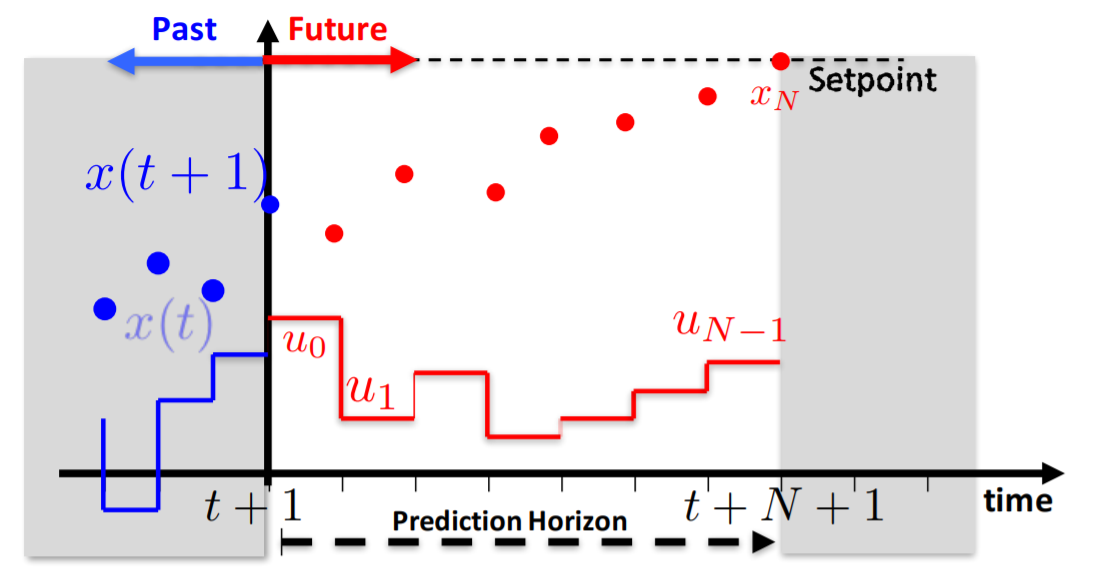
\includegraphics[width=0.6\textwidth]{MPC1.PNG}
	\caption{Visualization of the optimal control problem solved in one iteration of the MPC (Source: \cite{Patrinos2019}).}
	\label{fig:MPC1}
\end{figure}

\begin{figure}[h!]
	\centering
	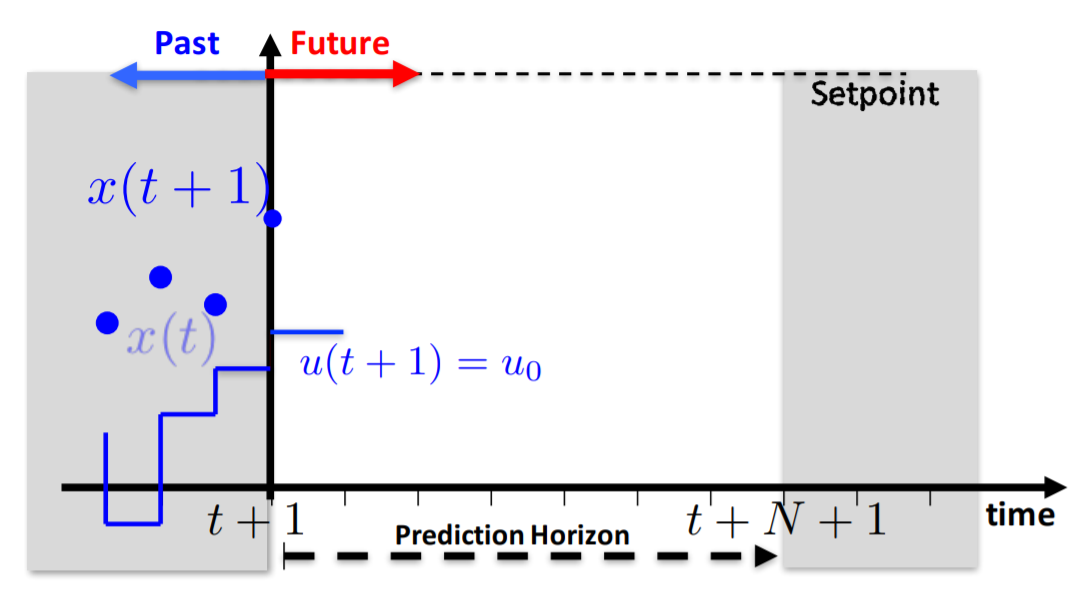
\includegraphics[width=0.6\textwidth]{MPC2.PNG}
	\caption{Visualization of the application of the first step of the calculated control signal during one iteration of the MPC (Source:\cite{Patrinos2019}).}
	\label{fig:MPC2}
\end{figure}

\newpage
\begin{equation}
\label{eq:MPC}
\begin{aligned}
\min_{\bm{q}(.),\bm{u}(.)} \quad & \sum_{k = 0}^{N-1}l_{k}(\bm{q}_{k},\bm{u}_{k}) + E(\bm{q}_{N}) \\
\textrm{s.t.} \quad & \bm{\dot{q}}_{k+1} = \sum_{k = 0}^{N-1}\bm{f}(\bm{q}_{k}, \bm{u}_{k})\\
& \bm{q}_{0}= \bm{q}_{measured}    \\
& h(\bm{q}_{k},\bm{u}_{k}) \geq 0	\\
& \bm{q}_{k}\in Q,\hspace{3 mm} \bm{u}_{k}\in U, \hspace{3 mm} N \in \mathbb{N}
\end{aligned}
\end{equation}




%\begin{equation}\label{eq:3}
%minimize_{\bm{q}(.),\bm{u}(.)}\sum_{k = 0}^{N-1}l_{k}(\bm{q}_{k},\bm{u}_{k}) + E(\bm{q}_{N})
%\end{equation}
%\hspace{42 mm} \textit{subject to:}
%\[\bm{\dot{q}}_{k+1} = \sum_{k = 0}^{N-1}\bm{f}(\bm{q}_{k}, \bm{u}_{k})\]
%\[\bm{q}_{0}= \bm{q}_{measured}\]
%\[h(\bm{q}_{k},\bm{u}_{k}) \geq 0\]
%\[\bm{q}_{k}\in Q,\hspace{3 mm} \bm{u}_{k}\in U, \hspace{3 mm} N \in \mathbb{N}\]


Equation \ref{eq:MPC} is a representation of the solved discrete system OCP during one iteration of the MPC. It is a discretized version of equation \ref{eq:OCP}. The Runge-Kutta integration is embedded in $\bm{f}$. The hard constraints are represented by $h$. It is worth noticing that the constraints can be violated in-between the different time sample points.\\

MPC has no direct feedback loop, but through the iterative way of solving the OCPs it can still deal with model mismatch or a changing environment. The downside of this approach is that it requires a bigger computational load, which makes efficiently written software a necessity. 


%%% Local Variables: 
%%% mode: latex
%%% TeX-master: "thesis"
%%% End: 